% SkillLens - CEN 3001 Advanced Computer Programming, FastAPI project presentation (Beamer, 16:9).
% Build: from docs/acp run  pdflatex slides.tex  (twice). Screenshots in figures/ come from
% scripts/acp_screenshots.py. Drafted with an AI assistant; the course lab lists AI coding assistants
% as allowed tools.
\documentclass[aspectratio=169,11pt]{beamer}
\usepackage[T1]{fontenc}
\usepackage[utf8]{inputenc}
\usepackage{lmodern}
\usepackage{amssymb}
\usepackage{booktabs}
\usepackage{listings}
\usepackage{tikz}
\usetikzlibrary{positioning,arrows.meta,fit,backgrounds,shadows,calc}
\graphicspath{{figures/}}

% ------------------------------------------------------------------ theme
\definecolor{navy}{HTML}{14213D}
\definecolor{navy2}{HTML}{2E4A7A}
\definecolor{accent}{HTML}{2A78D6}
\definecolor{soft}{HTML}{E8EEF8}
\definecolor{paper}{HTML}{F4F6FA}
\definecolor{good}{HTML}{2E7D4F}
\definecolor{warn}{HTML}{C0392B}
\definecolor{ink2}{HTML}{5B6476}

\setbeamertemplate{navigation symbols}{}
\setbeamercolor{normal text}{fg=navy}
\setbeamercolor{structure}{fg=accent}
\setbeamerfont{frametitle}{size=\Large,series=\bfseries}
\setbeamertemplate{itemize item}{\color{accent}\small$\blacksquare$}
\setbeamertemplate{enumerate item}{\tikz[baseline=(n.base)]\node[circle,fill=accent,text=white,inner sep=1.4pt,font=\scriptsize\bfseries](n){\insertenumlabel};}
\setbeamertemplate{frametitle}{%
  \begin{tikzpicture}[remember picture,overlay]
    \fill[navy] (current page.north west) rectangle ([yshift=-1.05cm]current page.north east);
    \fill[accent] ([yshift=-1.05cm]current page.north west) rectangle ([yshift=-1.12cm]current page.north east);
    \node[anchor=west,text=white,font=\Large\bfseries] at ([xshift=.55cm,yshift=-.53cm]current page.north west) {\insertframetitle};
  \end{tikzpicture}\vskip.9cm}
\setbeamertemplate{footline}{%
  \begin{tikzpicture}[remember picture,overlay]
    \node[anchor=south west,font=\tiny,text=ink2] at ([xshift=.4cm,yshift=.15cm]current page.south west)
      {SkillLens API \,·\, CEN 3001 Advanced Computer Programming \,·\, Rabia Demir};
    \node[anchor=south east,font=\tiny\bfseries,text=accent] at ([xshift=-.4cm,yshift=.15cm]current page.south east)
      {\insertframenumber/\inserttotalframenumber};
  \end{tikzpicture}}
\setbeamercolor{block title}{bg=navy,fg=white}
\setbeamercolor{block body}{bg=soft,fg=navy}
\setbeamertemplate{blocks}[rounded][shadow=false]

\lstset{basicstyle=\ttfamily\scriptsize, keywordstyle=\color{accent}\bfseries, commentstyle=\color{ink2},
  stringstyle=\color{good}, showstringspaces=false, frame=none, backgroundcolor=\color{paper},
  language=Python, columns=fullflexible, xleftmargin=4pt, framexleftmargin=4pt}

% a screenshot with a thin frame and a soft shadow
\newcommand{\shot}[2]{\tikz\node[inner sep=0pt,draw=navy!25,line width=.4pt,drop shadow={opacity=.18,shadow xshift=.6mm,shadow yshift=-.6mm}]{\includegraphics[width=#2]{#1}};}
% a big number with a caption
\newcommand{\bignum}[2]{\begin{tikzpicture}\node[fill=soft,rounded corners=3pt,minimum width=2.45cm,minimum height=1.4cm,align=center]
  {{\huge\bfseries\color{accent}#1}\\[1pt]{\scriptsize\color{ink2}#2}};\end{tikzpicture}}
% a coloured pill
\newcommand{\pill}[2]{\tikz[baseline=(p.base)]\node[fill=#1,text=white,rounded corners=5pt,inner sep=2.2pt,font=\scriptsize\bfseries](p){#2};}

\begin{document}

% ------------------------------------------------------------------ title
{\setbeamertemplate{footline}{}
\begin{frame}[plain]
\begin{tikzpicture}[remember picture,overlay]
  \fill[navy] (current page.south west) rectangle (current page.north east);
  \fill[accent] ([yshift=1.75cm]current page.south west) rectangle ([yshift=1.83cm]current page.south east);
  \node[anchor=east] at ([xshift=-.55cm,yshift=.6cm]current page.east)
    {\tikz\node[inner sep=0pt,draw=white,line width=1pt]{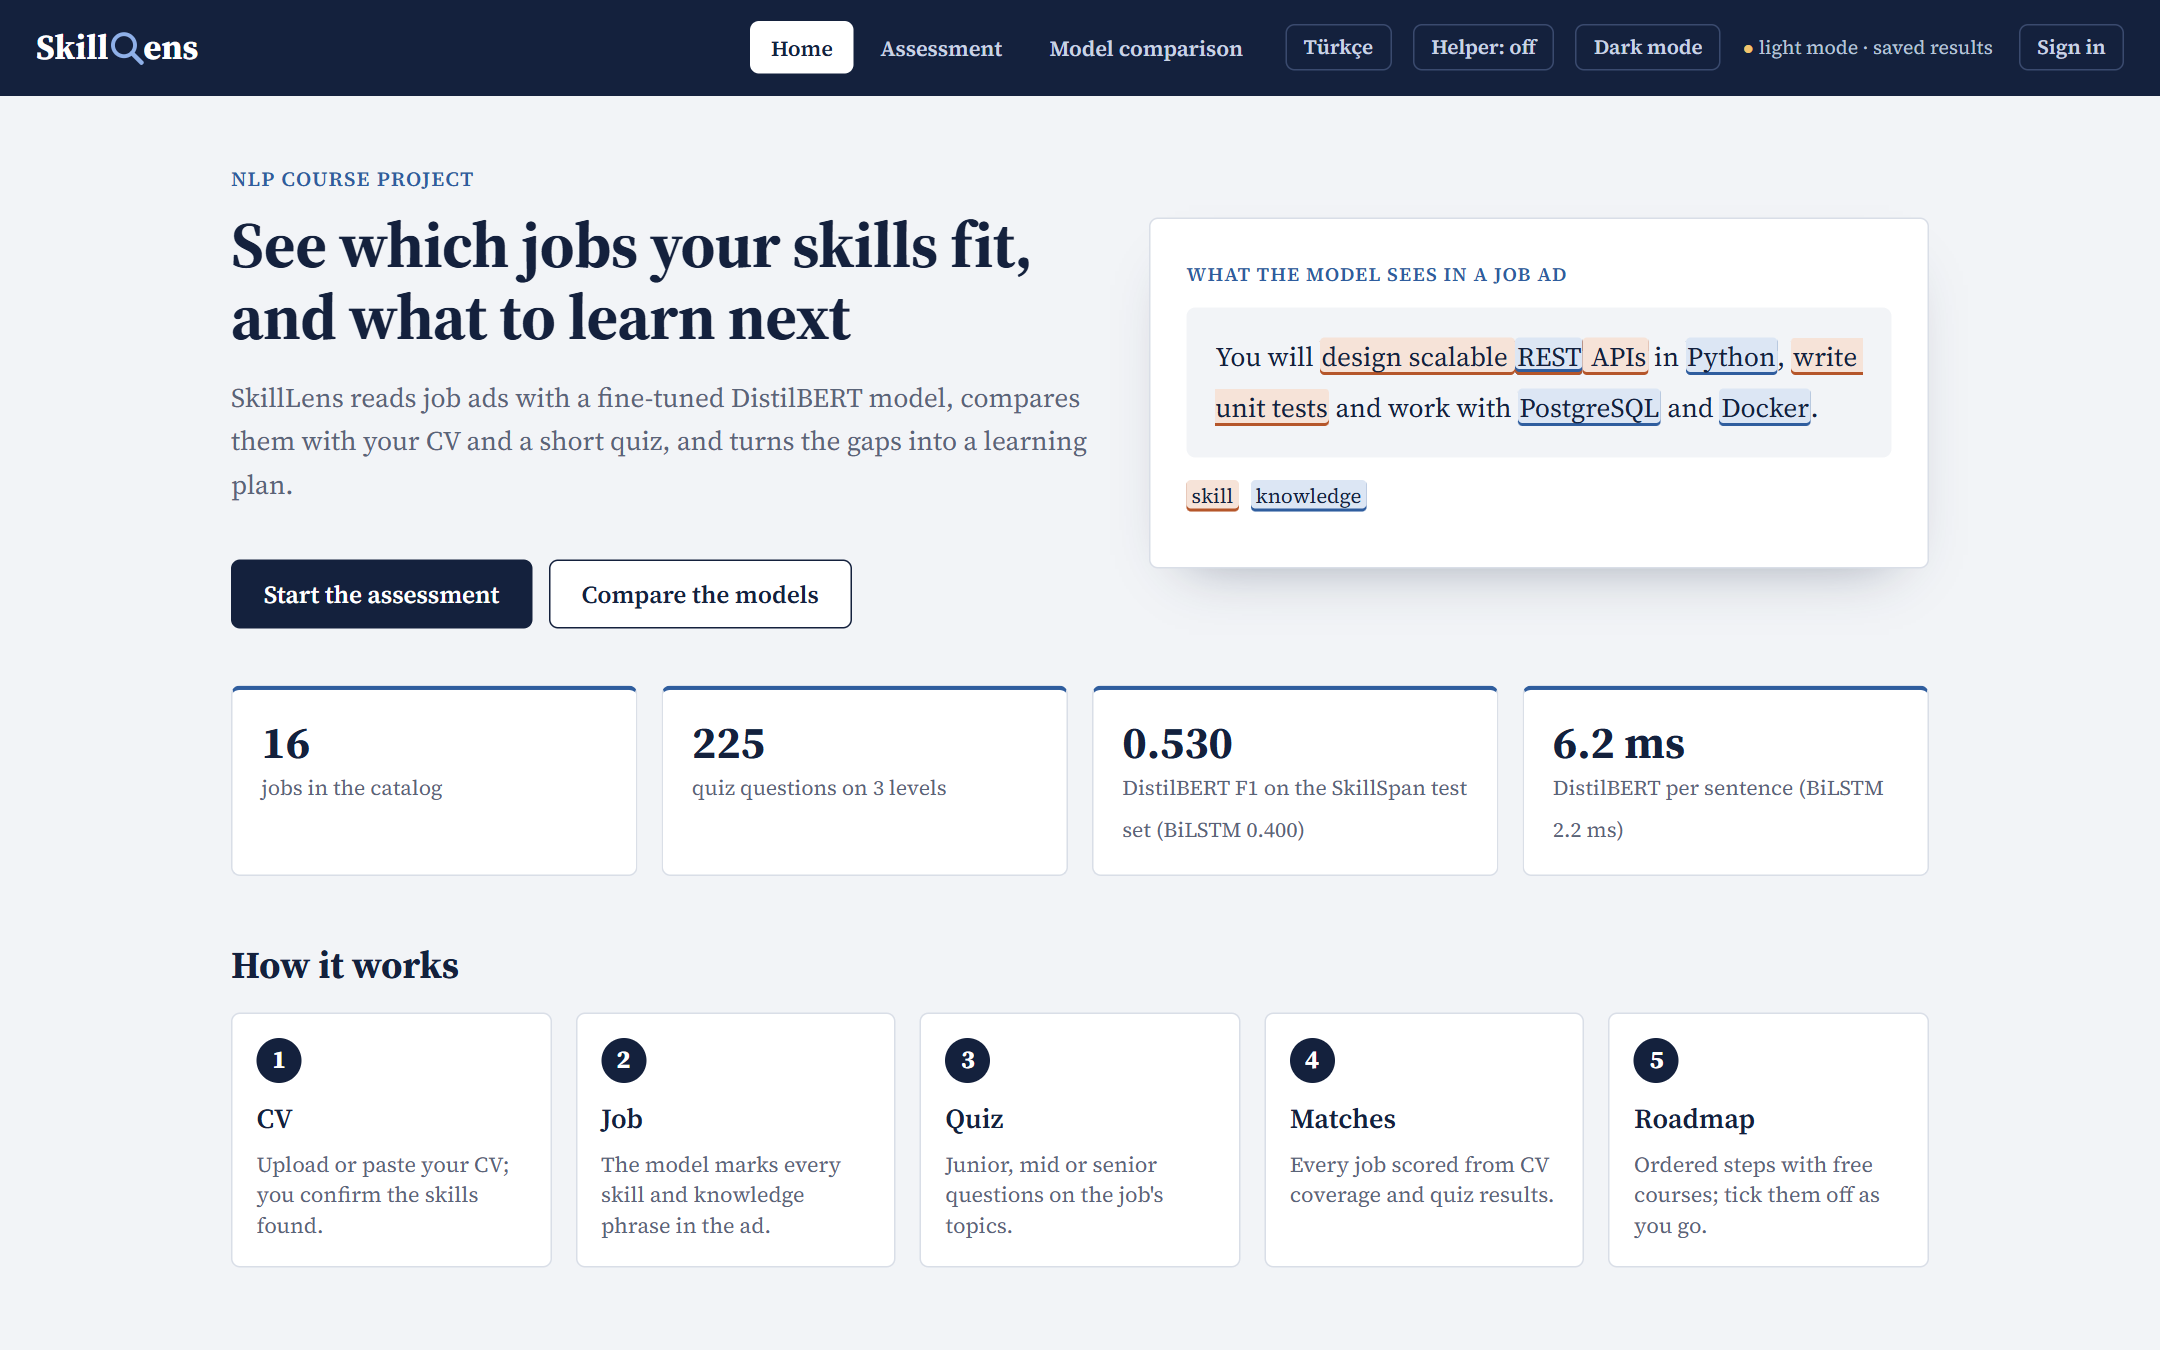
\includegraphics[width=6.4cm]{home.png}};};
  \node[anchor=west,text=white,font=\fontsize{38}{42}\selectfont\bfseries] at ([xshift=.9cm,yshift=1.75cm]current page.west) {SkillLens API};
  \node[anchor=west,text=soft,font=\large,align=left,text width=7.2cm] at ([xshift=.9cm,yshift=.45cm]current page.west)
    {Developer skill assessment and job matching, built on FastAPI};
  \node[anchor=west] at ([xshift=.9cm,yshift=-.75cm]current page.west)
    {\pill{accent}{FastAPI}\, \pill{navy2}{SQLModel}\, \pill{navy2}{JWT}\, \pill{navy2}{SQLite}\, \pill{good}{102 tests}};
  \node[anchor=south west,text=white,font=\small,align=left] at ([xshift=.9cm,yshift=.35cm]current page.south west)
    {\textbf{Rabia Demir} \,(22092090028)\\[2pt]
     {\color{soft}CEN 3001 Advanced Computer Programming \,·\, Haliç University \,·\, 25 November 2026}};
\end{tikzpicture}
\end{frame}}

% ------------------------------------------------------------------
\begin{frame}{What SkillLens does}
\begin{columns}[c]
\column{0.42\textwidth}
\begin{enumerate}\setlength\itemsep{3pt}
  \item Reads your \textbf{CV} and lists your skills
  \item Recommends \textbf{jobs} that fit the CV
  \item A short \textbf{quiz} checks what the CV claims
  \item A \textbf{match score} for every job
  \item A \textbf{learning roadmap} for the gaps
\end{enumerate}
\vspace{4pt}
\small A trained NLP model reads the job ads;\\ FastAPI serves the API \emph{and} the web app.
\column{0.56\textwidth}
\shot{jobs.png}{\linewidth}
\end{columns}
\vspace{4pt}
\centering
\bignum{9}{routers}\hspace{.15cm}\bignum{43}{API operations}\hspace{.15cm}\bignum{7}{database tables}\hspace{.15cm}\bignum{102}{automated tests}
\end{frame}

% ------------------------------------------------------------------
\begin{frame}{Architecture}
\centering
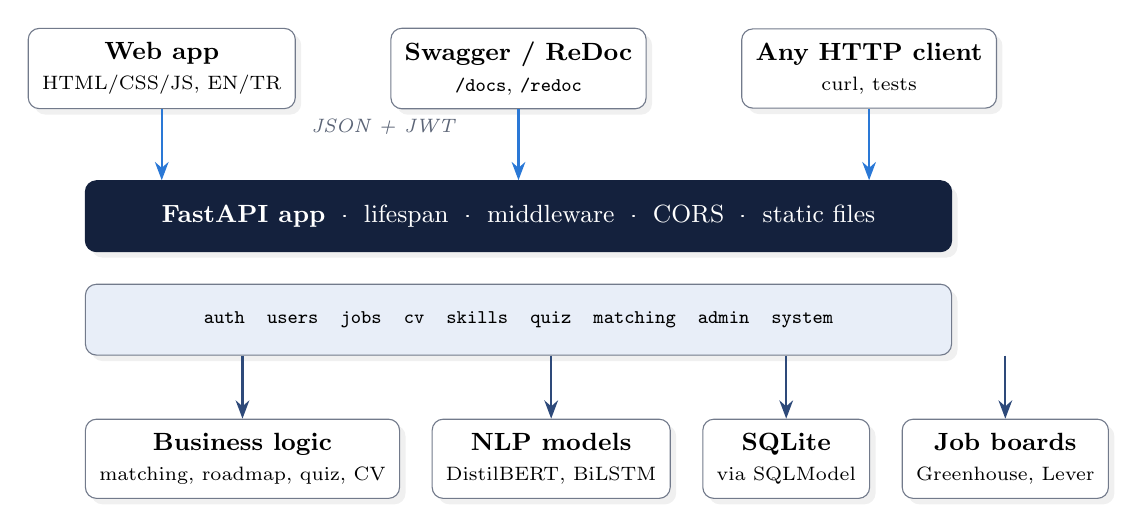
\begin{tikzpicture}[node distance=6mm and 9mm, >=Stealth, font=\small,
  box/.style={draw=navy!60, rounded corners=4pt, minimum height=9mm, inner sep=5pt, align=center, fill=white,
              drop shadow={opacity=.12}},
  hi/.style={box, fill=navy, text=white, draw=navy}]
  \node[box] (web) {\textbf{Web app}\\\scriptsize HTML/CSS/JS, EN/TR};
  \node[box, right=12mm of web] (docs) {\textbf{Swagger / ReDoc}\\\scriptsize \texttt{/docs}, \texttt{/redoc}};
  \node[box, right=12mm of docs] (curl) {\textbf{Any HTTP client}\\\scriptsize curl, tests};
  \node[hi, below=9mm of docs, minimum width=11cm] (api) {\textbf{FastAPI app} \;·\; lifespan \;·\; middleware \;·\; CORS \;·\; static files};
  \node[box, below=4mm of api, minimum width=11cm, fill=soft] (routers) {\scriptsize
    \texttt{auth}\quad \texttt{users}\quad \texttt{jobs}\quad \texttt{cv}\quad \texttt{skills}\quad \texttt{quiz}\quad \texttt{matching}\quad \texttt{admin}\quad \texttt{system}};
  \node[box, below=8mm of routers.south west, anchor=north west] (core) {\textbf{Business logic}\\\scriptsize matching, roadmap, quiz, CV};
  \node[box, right=4mm of core] (ml) {\textbf{NLP models}\\\scriptsize DistilBERT, BiLSTM};
  \node[box, right=4mm of ml] (db) {\textbf{SQLite}\\\scriptsize via SQLModel};
  \node[box, right=4mm of db] (ext) {\textbf{Job boards}\\\scriptsize Greenhouse, Lever};
  \foreach \n in {web,docs,curl} \draw[->, accent, thick] (\n) -- (\n |- api.north);
  \foreach \n in {core,ml,db,ext} \draw[->, navy2, thick] (routers.south -| \n) -- (\n);
  \node[font=\scriptsize\itshape, text=ink2, right=2pt of web.south east, anchor=north west] {JSON + JWT};
\end{tikzpicture}
\end{frame}

% ------------------------------------------------------------------
\begin{frame}[fragile]{Project structure}
\begin{columns}[T]
\column{0.5\textwidth}
\begin{lstlisting}[language={}]
main.py            entry for `fastapi dev`
api/
  main.py          app, lifespan, middleware
  state.py         shared state, dependencies
  security.py      Argon2 hashing, JWT
  schemas.py       request / response models
  routers/         auth users jobs cv skills
                   quiz matching admin system
core/
  db.py            SQLModel tables
  jobs.py          job store, importers
  matching.py roadmap.py quiz.py ...
web/               frontend (+ account.js)
tests/             pytest + TestClient
\end{lstlisting}
\column{0.46\textwidth}
\begin{block}{Design rules}
\small
\begin{itemize}
  \item One \textbf{router} per area, with its own tag in the docs
  \item Routers stay thin: validation in \texttt{schemas.py}, logic in \texttt{core/}
  \item Shared things are \textbf{dependencies}: DB session, current user, language, admin check
  \item Start: \texttt{fastapi dev main.py}
\end{itemize}
\end{block}
\end{columns}
\end{frame}

% ------------------------------------------------------------------
\begin{frame}{43 operations in 9 routers}
\begin{columns}[c]
\column{0.5\textwidth}
\scriptsize
\renewcommand{\arraystretch}{1.3}
\begin{tabular}{@{}l c p{4.3cm}@{}}
\toprule
\textbf{Router} & \textbf{Ops} & \textbf{Examples} \\
\midrule
\pill{good}{auth} & 2 & register, token (OAuth2 password) \\
\pill{accent}{users} & 14 & me, profile, quiz results, roadmaps, saved jobs \\
\pill{accent}{jobs} & 7 & list + filters, POST, PUT, PATCH, DELETE, import \\
\pill{navy2}{cv} & 2 & PDF upload, pasted text \\
\pill{navy2}{skills} & 3 & dictionary, extract, compare models \\
\pill{navy2}{quiz} & 3 & topics, start, submit \\
\pill{navy2}{matching} & 3 & matches, roadmap, roadmap PDF \\
\pill{warn}{admin} & 7 & stats, users, jobs, imports, questions \\
\pill{ink2}{system} & 2 & health, model results \\
\bottomrule
\end{tabular}
\column{0.48\textwidth}
\shot{docs.png}{\linewidth}
\end{columns}
\end{frame}

% ------------------------------------------------------------------
\begin{frame}{Database: SQLite through SQLModel}
\centering
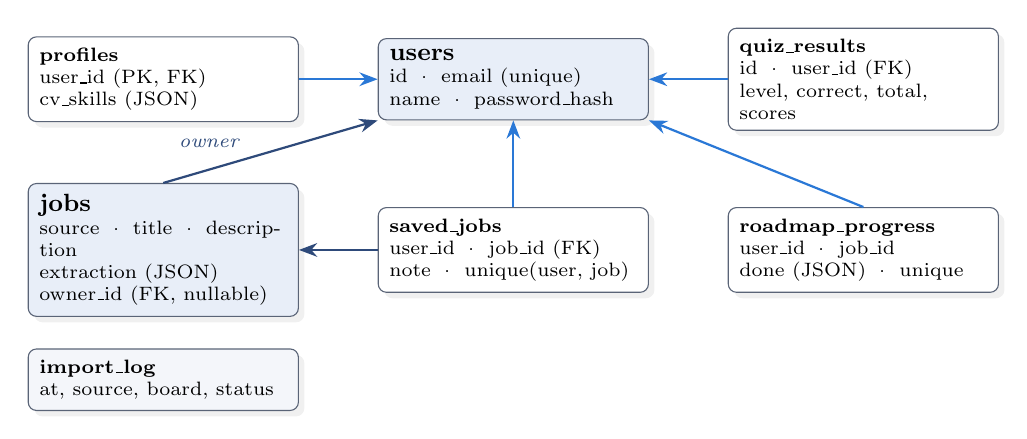
\begin{tikzpicture}[font=\scriptsize, >=Stealth,
  tbl/.style={draw=navy!70, rounded corners=3pt, align=left, inner sep=4pt, fill=white, text width=3.15cm,
              drop shadow={opacity=.12}},
  key/.style={tbl, fill=soft}]
  \node[key] (users) {\textbf{\small users}\\id \;·\; email (unique)\\name \;·\; password\_hash};
  \node[tbl, left=10mm of users] (profiles) {\textbf{profiles}\\user\_id (PK, FK)\\cv\_skills (JSON)};
  \node[tbl, right=10mm of users] (quiz) {\textbf{quiz\_results}\\id \;·\; user\_id (FK)\\level, correct, total, scores};
  \node[tbl, below=11mm of users] (saved) {\textbf{saved\_jobs}\\user\_id \;·\; job\_id (FK)\\note \;·\; unique(user, job)};
  \node[key, left=10mm of saved] (jobs) {\textbf{\small jobs}\\source \;·\; title \;·\; description\\extraction (JSON)\\owner\_id (FK, nullable)};
  \node[tbl, right=10mm of saved] (road) {\textbf{roadmap\_progress}\\user\_id \;·\; job\_id\\done (JSON) \;·\; unique};
  \node[tbl, below=4mm of jobs, fill=paper] (log) {\textbf{import\_log}\\at, source, board, status};
  \draw[->, thick, accent] (profiles) -- (users);
  \draw[->, thick, accent] (quiz) -- (users);
  \draw[->, thick, accent] (saved) -- (users);
  \draw[->, thick, accent] (road.north) -- (users.south east);
  \draw[->, thick, navy2] (jobs.north) -- node[above left, pos=.4, font=\scriptsize\itshape] {owner} (users.south west);
  \draw[->, thick, navy2] (saved) -- (jobs);
\end{tikzpicture}

\vspace{4pt}
\small Opens in the VS Code \textbf{SQLite Viewer}. An older database is upgraded at start:
missing tables are created and \texttt{jobs.owner\_id} is added.
\end{frame}

% ------------------------------------------------------------------
\begin{frame}{Sign-in and authorization}
\begin{columns}[c]
\column{0.56\textwidth}
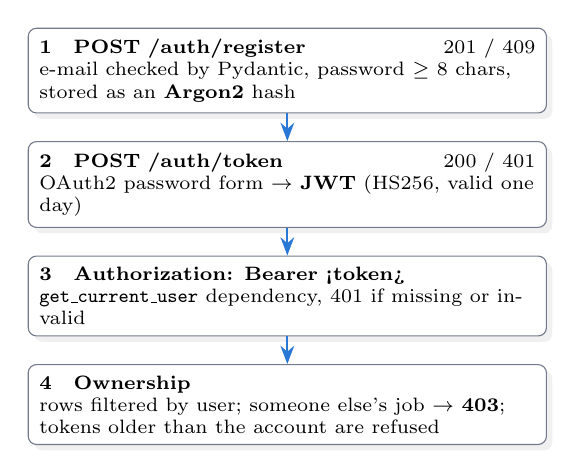
\begin{tikzpicture}[>=Stealth, font=\scriptsize, node distance=3.5mm,
  st/.style={draw=navy!60, fill=white, rounded corners=3pt, inner sep=4pt, text width=6.3cm, align=left,
             drop shadow={opacity=.12}}]
  \node[st] (a) {\textbf{1 \; POST /auth/register} \hfill 201 / 409\\ e-mail checked by Pydantic, password $\ge$ 8 chars, stored as an \textbf{Argon2} hash};
  \node[st, below=of a] (b) {\textbf{2 \; POST /auth/token} \hfill 200 / 401\\ OAuth2 password form $\rightarrow$ \textbf{JWT} (HS256, valid one day)};
  \node[st, below=of b] (c) {\textbf{3 \; Authorization: Bearer <token>}\\ \texttt{get\_current\_user} dependency, 401 if missing or invalid};
  \node[st, below=of c] (d) {\textbf{4 \; Ownership}\\ rows filtered by user; someone else's job $\rightarrow$ \textbf{403}; tokens older than the account are refused};
  \foreach \x/\y in {a/b,b/c,c/d} \draw[->, thick, accent] (\x) -- (\y);
\end{tikzpicture}
\column{0.42\textwidth}
\shot{signin.png}{\linewidth}

\vspace{4pt}
\scriptsize The same \texttt{/auth/token} endpoint powers the \textbf{Authorize} button in \texttt{/docs}.
\end{columns}
\end{frame}

% ------------------------------------------------------------------
\begin{frame}[fragile]{CRUD with ownership: jobs}
\begin{columns}[T]
\column{0.54\textwidth}
\scriptsize
\renewcommand{\arraystretch}{1.35}
\begin{tabular}{@{}l l l@{}}
\toprule
\textbf{Request} & \textbf{Who} & \textbf{Result} \\
\midrule
\texttt{GET /jobs?skill=Python\&limit=5} & anyone & \pill{good}{200} + total header \\
\texttt{POST /jobs} & signed in & \pill{good}{201} owner = caller \\
\texttt{PATCH /jobs/\{id\}} & owner & \pill{good}{200} sent fields only \\
\texttt{PUT /jobs/\{id\}} & owner & \pill{good}{200} text read again \\
\texttt{PATCH /jobs/\{id\}} & other user & \pill{warn}{403} \\
\texttt{DELETE} a demo job & signed in & \pill{warn}{403} read-only \\
\texttt{DELETE /jobs/\{id\}} & owner & \pill{good}{204} then \pill{warn}{404} \\
\bottomrule
\end{tabular}

\vspace{4pt}
Every row is an assertion in \texttt{tests/test\_users.py}.
\column{0.44\textwidth}
\begin{lstlisting}
@router.patch("/{job_id}",
              response_model=JobSummary)
def jobs_patch(job_id: int, body: JobPatch,
        user: User = Depends(get_current_user),
        lang: str = Depends(get_lang)):
    _own_job(job_id, user, lang)  # 404 / 403
    changes = body.model_dump(exclude_unset=True)
    return summary(
        state.store.update(job_id, changes))
\end{lstlisting}
\end{columns}
\end{frame}

% ------------------------------------------------------------------
\begin{frame}{FastAPI features used}
\begin{columns}[T]
\column{0.32\textwidth}
\begin{block}{Structure}
\scriptsize
\begin{itemize}
  \item \textbf{APIRouter}, prefixes, tags
  \item \textbf{Depends}: session, user, language, admin
  \item \textbf{lifespan}: DB, model, secrets
  \item \texttt{fastapi dev} entry point
\end{itemize}
\end{block}
\column{0.32\textwidth}
\begin{block}{Data and validation}
\scriptsize
\begin{itemize}
  \item \textbf{Pydantic} models, \texttt{response\_model}
  \item \texttt{EmailStr}, length and query limits
  \item \textbf{SQLModel} tables and sessions
  \item 201 / 204 / 401 / 403 / 404 / 409 / 422
\end{itemize}
\end{block}
\column{0.32\textwidth}
\begin{block}{Platform}
\scriptsize
\begin{itemize}
  \item HTTP \textbf{middleware}: calls and time per route
  \item \textbf{background task}: scheduled import
  \item \textbf{UploadFile}, PDF response
  \item \textbf{StaticFiles}, optional \textbf{CORS}
\end{itemize}
\end{block}
\end{columns}
\vspace{6pt}
\centering\shot{docs_jobs.png}{.56\textwidth}
\end{frame}

% ------------------------------------------------------------------
\begin{frame}{The web app on top of the API}
\begin{columns}[T]
\column{0.49\textwidth}
\shot{cv.png}{\linewidth}\\[4pt]
\scriptsize\textbf{CV} is scanned automatically; every skill shows the CV line it came from.
\column{0.49\textwidth}
\shot{job.png}{\linewidth}\\[4pt]
\scriptsize\textbf{Job ad} as the model read it; saved with the star when signed in.
\end{columns}
\end{frame}

\begin{frame}{Matches and the learning roadmap}
\begin{columns}[T]
\column{0.49\textwidth}
\shot{matches.png}{\linewidth}\\[4pt]
\scriptsize\textbf{Matches}: most requested skills, coloured by the user's evidence; profile panel on the right.
\column{0.49\textwidth}
\shot{roadmap.png}{\linewidth}\\[4pt]
\scriptsize\textbf{Roadmap}: ordered steps with free courses; ticks are saved per user on the server.
\end{columns}
\end{frame}

% ------------------------------------------------------------------
\begin{frame}{Running it: full mode and light mode}
\begin{columns}[T]
\column{0.48\textwidth}
\begin{block}{Two ways to start}
\scriptsize
\renewcommand{\arraystretch}{1.25}
\begin{tabular}{@{}l l l@{}}
 & \textbf{Full} & \textbf{Light} \\
\midrule
NLP models & loaded & not loaded \\
Start time & about 1 min & about 4 s \\
Job pages & live model & saved results \\
New text & yes & no (clear 503) \\
\end{tabular}
\end{block}
\scriptsize Light mode: \texttt{SKILLLENS\_LIGHT=1}; \texttt{/health} reports the mode.

\vspace{4pt}
\begin{block}{For the demo}
\scriptsize
\begin{itemize}
  \item One command starts the app and a public \textbf{https} link
  \item \texttt{seed\_demo\_account.py}: demo user with saved data
\end{itemize}
\end{block}
\column{0.5\textwidth}
\shot{admin.png}{\linewidth}\\[4pt]
\scriptsize\textbf{Admin page}: jobs, imports, question bank, API calls and average time per route.
\end{columns}
\end{frame}

% ------------------------------------------------------------------
\begin{frame}{Testing}
\begin{columns}[c]
\column{0.34\textwidth}
\centering
\bignum{102}{tests pass}\\[8pt]
\scriptsize\texttt{python -m pytest -q tests}
\column{0.64\textwidth}
\small
\begin{itemize}\setlength\itemsep{3pt}
  \item \texttt{pytest} + FastAPI \textbf{TestClient}; each test uses its own temporary SQLite file
  \item A fake tagger replaces the neural model, so API tests need no GPU
  \item Sign-up, sign-in, bad and missing tokens, \textbf{one user cannot read another's data}
  \item Job CRUD and ownership, filters, pagination, account deletion
  \item Light mode, demo account, OpenAPI tags and security scheme
  \item Admin API, CV upload errors, quiz, matching, roadmap
\end{itemize}
\end{columns}
\end{frame}

% ------------------------------------------------------------------
\begin{frame}{Live demo}
\begin{columns}[T]
\column{0.5\textwidth}
\begin{enumerate}\setlength\itemsep{5pt}
  \item \texttt{/docs}: routers, schemas, \textbf{Authorize}
  \item \texttt{GET /users/me} with the demo account
  \item \texttt{POST} a job, \texttt{PATCH} it, \texttt{DELETE} it; 403 for another user
\end{enumerate}
\column{0.5\textwidth}
\begin{enumerate}\setcounter{enumi}{3}\setlength\itemsep{5pt}
  \item Web app: sign in, sample CV, recommended jobs, star a job
  \item Quiz $\rightarrow$ matches $\rightarrow$ roadmap; reload: data comes back
  \item Database in the SQLite Viewer, admin page
\end{enumerate}
\end{columns}
\vspace{14pt}
\centering

\begin{tikzpicture}
  \node[fill=navy,text=white,rounded corners=4pt,inner sep=8pt,font=\small]
    {Source code: \textbf{github.com/rabiaddd3-prog/skillens-with-fastapi}};
\end{tikzpicture}
\end{frame}

% ------------------------------------------------------------------
\begin{frame}{Summary}
\begin{columns}[T]
\column{0.55\textwidth}
\begin{block}{What was built}
\small
\begin{itemize}
  \item FastAPI service: 9 routers, 43 operations
  \item SQLite through SQLModel, 7 tables
  \item Argon2 passwords, JWT sign-in, per-user data, ownership checks
  \item Bilingual web app with an NLP model inside
  \item 102 automated tests
\end{itemize}
\end{block}
\column{0.42\textwidth}
\begin{block}{Limitations}
\small
\begin{itemize}
  \item One SQLite file: fine for a prototype, not for many writers
  \item JWTs cannot be revoked before they expire
  \item No e-mail check or rate limiting
  \item Tested on Python 3.11
\end{itemize}
\end{block}
\end{columns}
\vspace{16pt}
\centering{\Large\bfseries\color{accent}Thank you!}\\[3pt]{\small\color{ink2}Questions?}
\end{frame}

\end{document}
